\documentclass{article}

\usepackage[T1]{fontenc}    %Schriftart des Dokumentes
\usepackage[ngerman]{babel} %Dokumentensprache, hier Deutsch
\usepackage{amsmath, amssymb, stmaryrd} %mathematische Schriftzeichen
\usepackage{graphicx} %Einfügen von Grafiken
\usepackage{wrapfig}
\usepackage{bm}
\usepackage{subfig}
\usepackage{newclude}
\usepackage{pdfpages}

\setlength{\parindent}{0pt} %Einrückung von Absätzen auf null gesetzt
\setlength{\parskip}{10pt} %Abstand zischen Absätzen auf 10pt gesetzt

\title{Versuch 211: Gekoppelte Pendel}
\author{Matthias Kuntz}
\date{21.02.2024}

\renewcommand*\contentsname{Zusammenfassung}

\begin{document}

\maketitle

\tableofcontents

\newpage

%-------------------------EINLEITUNG-------------------------
\section{Einleitung}

Eines der wichtigsten in der Physik beschriebenen Phänomene sind gekoppelte, schwingungsfähige Systeme. Seien es Atomgruppen innerhalb eines Moleküls, die elektromagnetischen Verbindungen einer Kristallstruktur oder sogar die Herzschrittmacherzellen im menschlichen Körper. All diesen Systemen liegt ein gekoppeltes Schwingsystem zugrunde. Ziel dieses Versuches ist, anhand der Betrachtung eines einfachen Systems von zwei gekoppelten Schwingpendeln die Grundlagen der Kopplung sowie verschwiedene Schwingtypen zu verstehen und analysieren.  

\subsection{Physikalische Grundlagen}

\subsubsection{Bewegung schwingender Pendel}

Die Beschreibung eines einfachen ungekoppelten Schwingpendels lässt sich einfach als harmonischer Oszillator herleiten. Für ein Pendel mit Trägheitsmoment $J$, Direktionsmoment $D = mgL$, Masse $m$ und Pendellänge $L$, $g$ ist wie gewohnt die Erdbeschleunigung, gilt für kleine Winkelauslenkungen $\phi$:

\begin{equation}
    J \ddot{\phi} + D \phi = 0.
    \label{eq:einfach_ungekoppeltes_Pendel}
\end{equation}

Die Lösung ist hierbei altbekannt eine harmonische Schwingung mit der Kreisfrequenz

\begin{equation}
    \omega = \sqrt{\frac{D}{J}} = \sqrt{\frac{g}{L}}.
    \label{eq:kreisfreq_harm}
\end{equation}

Werden nun zwei solche Pendel über eine Feder aneinandergekoppelt, so kann der Feder das zusätzliche Direktionsmoment $D' = D_F l^2$ zugewiesen werden, wobei $D_F$ die Federkonstante und $l$ die Länge der Feder bezeichnen. Somit wirken die zusätzlichen Drehmomente $M_1 = D' (\phi_2 - \phi_1)$ auf Pendel 1 sowie $M_2 = D' (\phi_1 - \phi_2)$ auf Pendel 2 und es ergibt sich das folgende System gekoppelter Differentialgleichungen:

\begin{equation}
    \begin{split}
        J \ddot{\phi}_1 &= -D \phi_1 + D' (\phi_2 - \phi_1) \\
        J \ddot{\phi}_2 &= -D \phi_2 + D' (\phi_1 - \phi_2).
    \end{split}
\end{equation}

Dieses System kann man lösen, indem man die beiden Gleichungen $\ddot{\phi}_1 + \ddot{\phi}_2$ sowie $\ddot{\phi}_1 - \ddot{\phi}_2$ bestimmt und diese mit den Substitutionen $u = \phi_1 + \phi_2$ und $v = \phi_1 - \phi_2$ zu zwei unabhängigen Gleichungen für $u$ und $v$ entkoppelt. Man erhält die beiden Gleichungen

\begin{equation}
    \begin{split}
        J \ddot{u} &+ Du = 0 \\
        J \ddot{v} &+ (D +2D')v = 0,
    \end{split}
\end{equation}

deren Lösungen harmonische Schwingungen mit den Kreisfrequenzen $\omega_1$ und $\omega_2$ sind:

\begin{equation}
    \begin{split}
        u(t) &= A_1 \cos{(\omega_1 t)} + B_1 \sin{(\omega_1 t)} \ \ \ \ \text{mit} \ \ \omega_1 = \sqrt{\frac{D}{J}} \\
        v(t) &= A_2 \cos{(\omega_2 t)} + B_2 \sin{(\omega_2 t)} \ \ \ \ \text{mit} \ \ \omega_2 = \sqrt{\frac{D+2D'}{J}}.
    \end{split}
\end{equation}

Substituiert man wieder zurück zu $\phi_1$ und $\phi_2$ so erhält man die beiden Gleichen für die Auslenkungswinkel der Pendel.

\begin{equation}
    \begin{split}
        \phi_1 (t) &= \frac{1}{2} \left( A_1 \cos{(\omega_1 t)} + B_1 \sin{(\omega_1 t)} + A_2 \cos{(\omega_2 t)} + B_2 \sin{(\omega_2 t)} \right) \\
        \phi_2 (t) &= \frac{1}{2} \left( A_1 \cos{(\omega_1 t)} + B_1 \sin{(\omega_1 t)} - A_2 \cos{(\omega_2 t)} - B_2 \sin{(\omega_2 t)} \right)
    \end{split}
    \label{eq:EOMsKoppl}
\end{equation}

Im folgenden werden wir betrachten, wie verschiedene Anfangsbedingungen verschiedene Schwingtypen erzeugen und sich die Gleichungen nochmal deutlich vereinfachen.

\subsubsection{Symmetrische Schwingungen}

Werden beide Pendel am Anfang in die gleiche Richtung gleich weit ausgelenkt und zur gleichen Zeit ($t = 0$) mit derselben Startgeschwindigkeit ($\dot{\phi} = 0$) losgelassen, so entsteht eine symmetrische Schwingung. Diese Anfangsbedingungen lassen sich mathematisch Folgendermaßen formulieren:

\begin{equation}
    \begin{split}
        \phi_1 (0) &= \phi_2 (0) = \phi_0 \\
        \dot{\phi}_1 (0) &= \dot{\phi}_2 (0) = 0.
    \end{split}
\end{equation}

Vereinfacht man die Bewegungsgleichungen mit diesen Bedingen so erhält man:

\begin{equation}
    \phi_1(t) = \phi_2(t) = \phi_0 \cos{(\omega_1 t)}.
    \label{eq:EOMsymm}
\end{equation}

Es bewegen sich also beide Pendel exakt gleich mit $\omega_1$ und sind somit unabhängig von der Kopplung. Dies ist auch intuitiv, da bei der gleichförmigen symmetrischen Schwingung die Feder niemals gestreckt oder gestaucht wird.

\subsubsection{Antisymmetrische Schwingung}

Erneut müssen beide Pendel um den gleichen Anfangswert ausgelenkt werden, diesmal aber gegenphasig:

\begin{equation}
    \begin{split}
        \phi_1 (0) &= -\phi_2 (0) = \phi_0 \\
        \dot{\phi}_1 (0) &= \dot{\phi}_2 (0) = 0.
    \end{split}
\end{equation}

Mit diesen Bedingungen nehmen die Bewegungsgleichungen folgende Form an:

\begin{equation}
    \phi_1(t) = -\phi_2(t) = \phi_0 \cos{(\omega_2 t)}.
    \label{eq:EOMasymm}
\end{equation}

Somit schwingen die Pendel zwar immer noch mit gleicher Frequenz, nun aber gegenphasig mit der von der Kopplung abhängenden Frequenz $\omega_2$. Man kann es sich so vorstellen, dass die Feder die Schwingung antreibt, indem sie beim Gegeneinanderlaufen der beiden Pendel immer wieder gestaucht und gestreckt wird.

\subsubsection{Schwebungsschwingung}

Zu guter Letzt setzt die Schwebung voraus, dass das eine Pendel anfangs ausgelenkt wird, während das andere zunächst in der Ruhelage gehalten wird.

\begin{equation}
    \begin{split}
        \phi_1 (0) &=0, \ \ \ \ \phi_2 (0) = \phi_0 \\
        \dot{\phi}_1 (0) &= \dot{\phi}_2 (0) = 0.
    \end{split}
\end{equation}

Es entstehen die folgen Bewegungsgleichungen:

\begin{equation}
    \begin{split}
        \phi_1(t) &= \phi_0 \sin{(\omega_I t)} \sin{(\omega_{II} t)} \\
        \phi_2(t) &= \phi_0 \cos{(\omega_I t)} \cos{(\omega_{II} t)}.
    \end{split}
    \label{eq:EOMbeat}
\end{equation}

Neu definiert wurden hierbei die Frequenzen $\omega_I = \frac{1}{2}(\omega_2 + \omega_1)$, mit der beide Pendel einzel schwingen, sowie $\omega_{II} = \frac{1}{2}(\omega_2 - \omega_1)$, die sogenannte Schwebungsfrequenz, mit der die Energie eines Einzelpendels oszilliert. 

Bei einer Schwebung beginnt das am Anfang ausgelenkte Pendel nach und nach seine Schwingenergie über die Kopplung auf das andere Pendel zu übertragen, wodurch dieses zur Schwingung angeregt wird. Dieser Prozess geht soweit, bis praktisch die gesamte Energie im anderen Pendel steckt und ein Zustand erreicht wird, indem das anfänglich ausgelenkte Pendel ruht und das andere schwingt. An diesem Punkt kehrt sich der Prozess um.

Die Frequenzen $\omega_1$ und $\omega_2$ werden als Eigenfrequenzen der Schwingung bezeichnet und die zu diesen Eigenfrequenzen gehörenden Schwingungen werden wiederum als Normalschwingungen bezeichnet. Allgemein gilt, dass bei einem gekoppelten System von $N$ Oszillatoren $N$ Normalschwingungen existieren und jede mögliche Schwingung eines Oszillators sowie damit auch die Schwebungsschwingung selbst als Linearkombination dieser Normalschwingungen beschrieben werden kann. 

\subsubsection{Kopplungsgrad}

Der Kopplungsgrad $\kappa$ quantifiziert die Stärke einer Kopplung. Man kann ihn sowohl über die Direktionsmomente mit 

\begin{equation}
    \kappa = \frac{D'}{D + D'},
    \label{eq:KopplGr_D}
\end{equation}

als auch über die Frequenzen oder Periodendauer der Schwingung definieren:

\begin{equation}
    \kappa = \frac{\omega_2^2 - \omega_1^2}{\omega_2^2 + \omega_1^2} = \frac{T_2^2 - T_1^2}{T_2^2 + T_1^2}.
    \label{eq:KopplGr_wT}
\end{equation}

\subsubsection{Elektrischer Schwingkreis}

Ein weiteres gekoppeltes System ist der elektrische Schwingkreis. Hier werden zwei Spulen induktiv gekoppelt indem sie so nebeneinander gelegt werden, dass ihre Achsen auf einer Linie liegen. Befinden sich nun beide Spulen jeweils in einem eigenen Schwingkreis, bestehend aus der jeweiligen Spule und einem Kondensator, so kann man beobachten, dass eine im einen Schwingkreis angeregte Schwingung analog zum mechanischen Fall über die hier induktive Kopplung auf den anderen Schwingkreis übertragen wird. Somit beginnt der zweite Schwingkreis zu schwingen und die Schwingung im Ersten lässt nach, bis auch hier der Umkehrpunkt erreicht wird, an dem der erste Schwingkreis nicht mehr schwingt und nun wieder vom Zweiten angeregt wird, der nun die Rolle des ursprünglichen Schwingkreises übernimmt.     

\subsection{Versuchsaufbau}

Der Aufbau besteht aus zwei fest aufgehängten Pendeln, deren Auslenkung unter Verwendung des Hall-Effekts mithilfe einer Software digital aufgezeichnet werden kann. Ein Sensor in der Pendelachse misst hierbei die zum Sinus des Auslenkungswinkel proportionale Hall-Spannung, die dadurch entsteht, dass das in der Halterung angelegte Magnetfeld eine Spannung in dem sich drehenden Sensor induziert. An den Pendeln sind drei versiedenene Stellen, an denen die Kopplungsfeder angebracht werden kann, wodurch drei verschiedene Kopplungsgrade, schwach, mittel und stark, untersucht werden können. 

\phantom{.}

\begin{figure}[!h]
    \centering
    \includegraphics[width=0.9\textwidth]{graphics/Aufbau.png}
    \caption{Versuchsaufbau [Quelle: Skript PAP2.1, S. 2, Stand: 23.02.2024]}
    \label{fig:Aufbau}
\end{figure}

%---------------VERSUCHSPROTOKOLL MIT MESSDATEN---------------
\newpage

\section{Versuchsprotokoll mit Messdaten}

\includegraphics[width=\textwidth]{graphics/mess1.jpg}
\newpage
\includegraphics[width=\textwidth]{graphics/mess2.jpg}
\newpage
\includegraphics[width=\textwidth]{graphics/mess3.jpg}
\newpage

\addtocounter{table}{3}

\begin{figure}[p]
  \centering
  \subfloat[]{\includegraphics[width=0.8\textwidth]{graphics/messungen/uncoupled pendulums.png}\label{fig:uncoup_norm}}
  \hfill
  \subfloat[(FFT)]{\includegraphics[width=0.8\textwidth]{graphics/messungen/uncoupled pendulums_fft.png}\label{fig:uncoup_fft}}
  \hfill
  \caption{Gemessene ungekoppelte Schwingung}
  \label{fig:uncoup}
\end{figure}

\begin{figure}[p]
  \centering
  \subfloat[Schwache Kopplung]{\includegraphics[width=0.48\textwidth]{graphics/messungen/symmetric - weak coupling.png}\label{fig:symm_weak}}
  \hfill
  \subfloat[Schwache Kopplung (FFT)]{\includegraphics[width=0.48\textwidth]{graphics/messungen/symmetric - weak coupling_fft.png}\label{fig:symm_weak_fft}}
  \hfill
  \subfloat[Mittlere Kopplung]{\includegraphics[width=0.48\textwidth]{graphics/messungen/symmetric - middle coupling.png}\label{fig:symm_med}}
  \hfill
  \subfloat[Mittlere Kopplung (FFT)]{\includegraphics[width=0.48\textwidth]{graphics/messungen/symmetric - middle coupling_fft.png}\label{fig:symm_med_fft}}
  \hfill
  \hfill
  \subfloat[Starke Kopplung]{\includegraphics[width=0.48\textwidth]{graphics/messungen/symmetric - strong coupling.png}\label{fig:symm_stark}}
  \hfill
  \subfloat[Starke Kopplung (FFT)]{\includegraphics[width=0.48\textwidth]{graphics/messungen/symmetric - strong coupling_fft.png}\label{fig:symm_stark_fft}}
  \hfill
  \caption{Gemessene Symmetrische Swingungen}
  \label{fig:symmMess}
\end{figure}

\begin{figure}[p]
  \centering
  \subfloat[Schwache Kopplung]{\includegraphics[width=0.48\textwidth]{graphics/messungen/asymmetric - weak coupling.png}\label{fig:asymm_weak}}
  \hfill
  \subfloat[Schwache Kopplung (FFT)]{\includegraphics[width=0.48\textwidth]{graphics/messungen/asymmetric - weak coupling_fft.png}\label{fig:asymm_weak_fft}}
  \hfill
  \subfloat[Mittlere Kopplung]{\includegraphics[width=0.48\textwidth]{graphics/messungen/asymmetric - middle coupling.png}\label{fig:asymm_med}}
  \hfill
  \subfloat[Mittlere Kopplung (FFT)]{\includegraphics[width=0.48\textwidth]{graphics/messungen/asymmetric - middle coupling_fft.png}\label{fig:asymm_med_fft}}
  \hfill
  \hfill
  \subfloat[Starke Kopplung]{\includegraphics[width=0.48\textwidth]{graphics/messungen/asymmetric - strong coupling.png}\label{fig:asymm_stark}}
  \hfill
  \subfloat[Starke Kopplung (FFT)]{\includegraphics[width=0.48\textwidth]{graphics/messungen/asymmetric - strong coupling_fft.png}\label{fig:asymm_stark_fft}}
  \hfill
  \caption{Gemessene Antisymmetrische Swingungen}
  \label{fig:asymmMess}
\end{figure}

\begin{figure}[p]
  \centering
  \subfloat[Schwache Kopplung]{\includegraphics[width=0.48\textwidth]{graphics/messungen/beat - weak coupling.png}\label{fig:beat_weak}}
  \hfill
  \subfloat[Schwache Kopplung (FFT)]{\includegraphics[width=0.48\textwidth]{graphics/messungen/beat - weak coupling_fft.png}\label{fig:beat_weak_fft}}
  \hfill
  \subfloat[Mittlere Kopplung]{\includegraphics[width=0.48\textwidth]{graphics/messungen/beat - middle coupling.png}\label{fig:beat_med}}
  \hfill
  \subfloat[Mittlere Kopplung (FFT)]{\includegraphics[width=0.48\textwidth]{graphics/messungen/beat - middle coupling_fft.png}\label{fig:beat_med_fft}}
  \hfill
  \hfill
  \subfloat[Starke Kopplung]{\includegraphics[width=0.48\textwidth]{graphics/messungen/beat - strong coupling.png}\label{fig:beat_stark}}
  \hfill
  \subfloat[Starke Kopplung (FFT)]{\includegraphics[width=0.48\textwidth]{graphics/messungen/beat - strong coupling_fft.png}\label{fig:beat_stark_fft}}
  \hfill
  \caption{Gemessene Schwebungen}
  \label{fig:beatMess}
\end{figure}

\begin{figure}[p]
  \centering
  \subfloat[kein Abstand - siehe Bild 1]{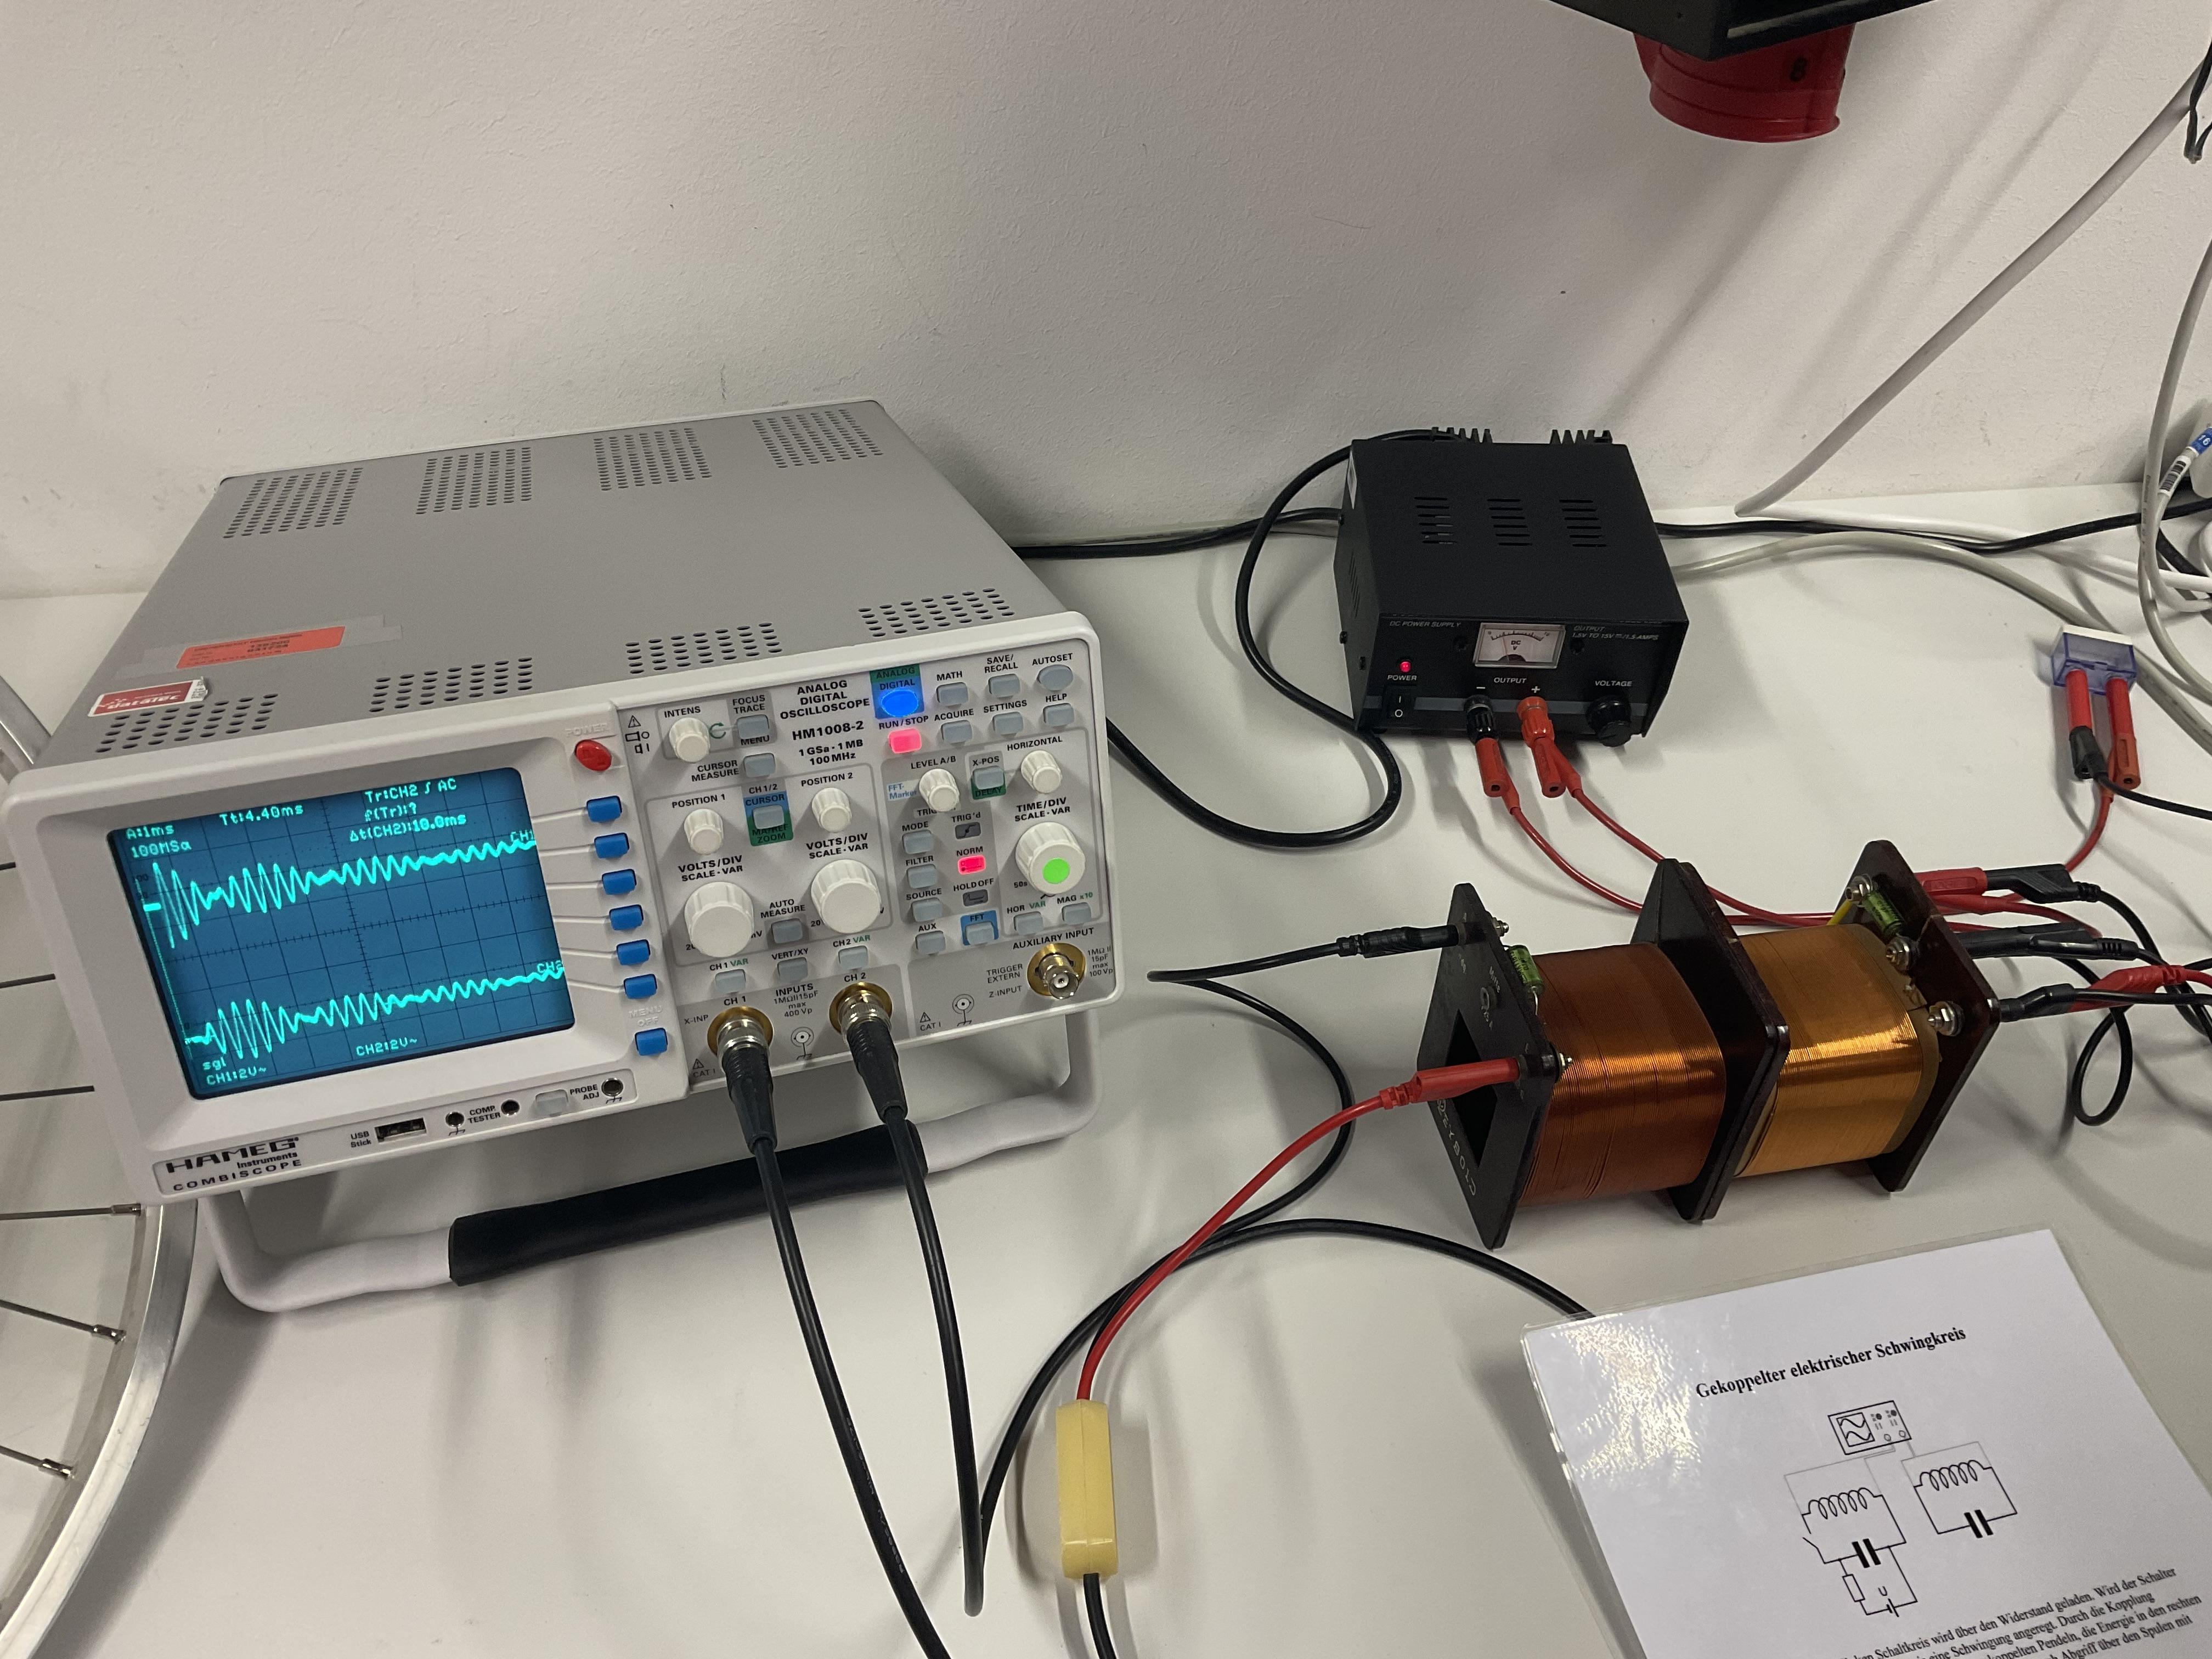
\includegraphics[width=0.48\textwidth]{graphics/IMG_0621.jpg}\label{fig:el_0}}
  \hfill
  \subfloat[kleiner Abstand - siehe Bild 2]{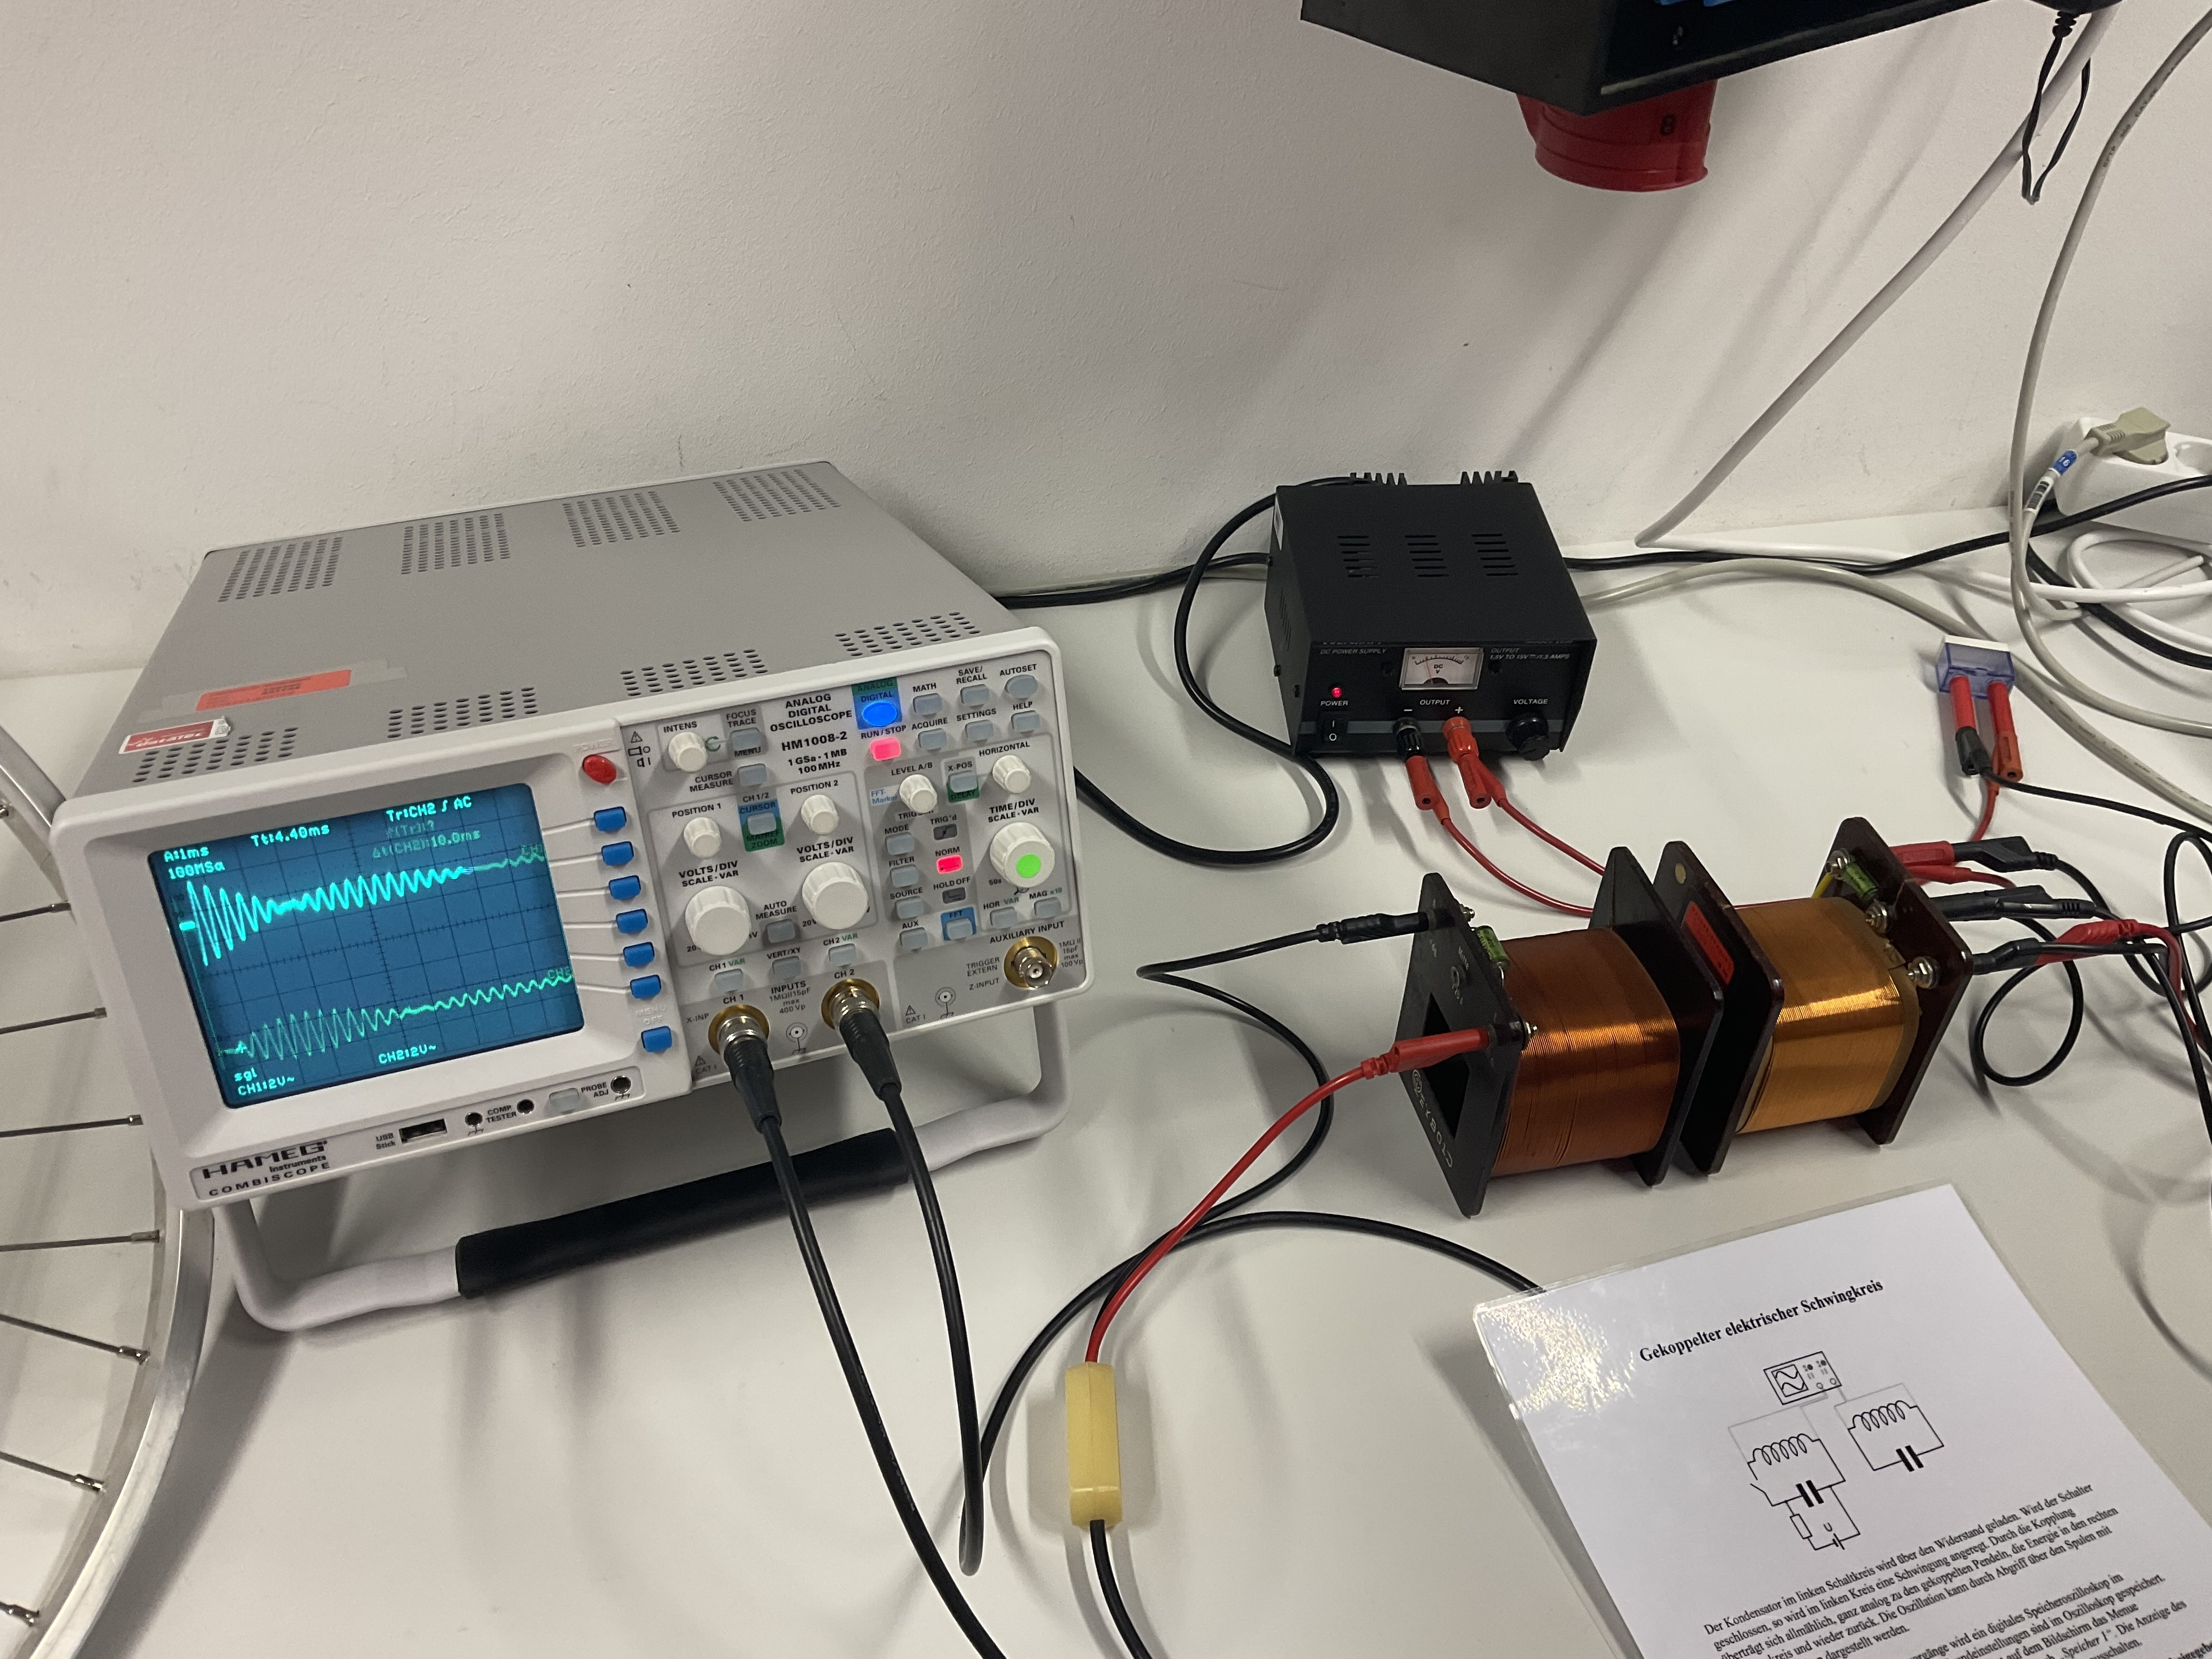
\includegraphics[width=0.48\textwidth]{graphics/IMG_0622.jpg}\label{fig:el_klein}}
  \hfill
  \subfloat[großer Abstand - siehe Bild 3]{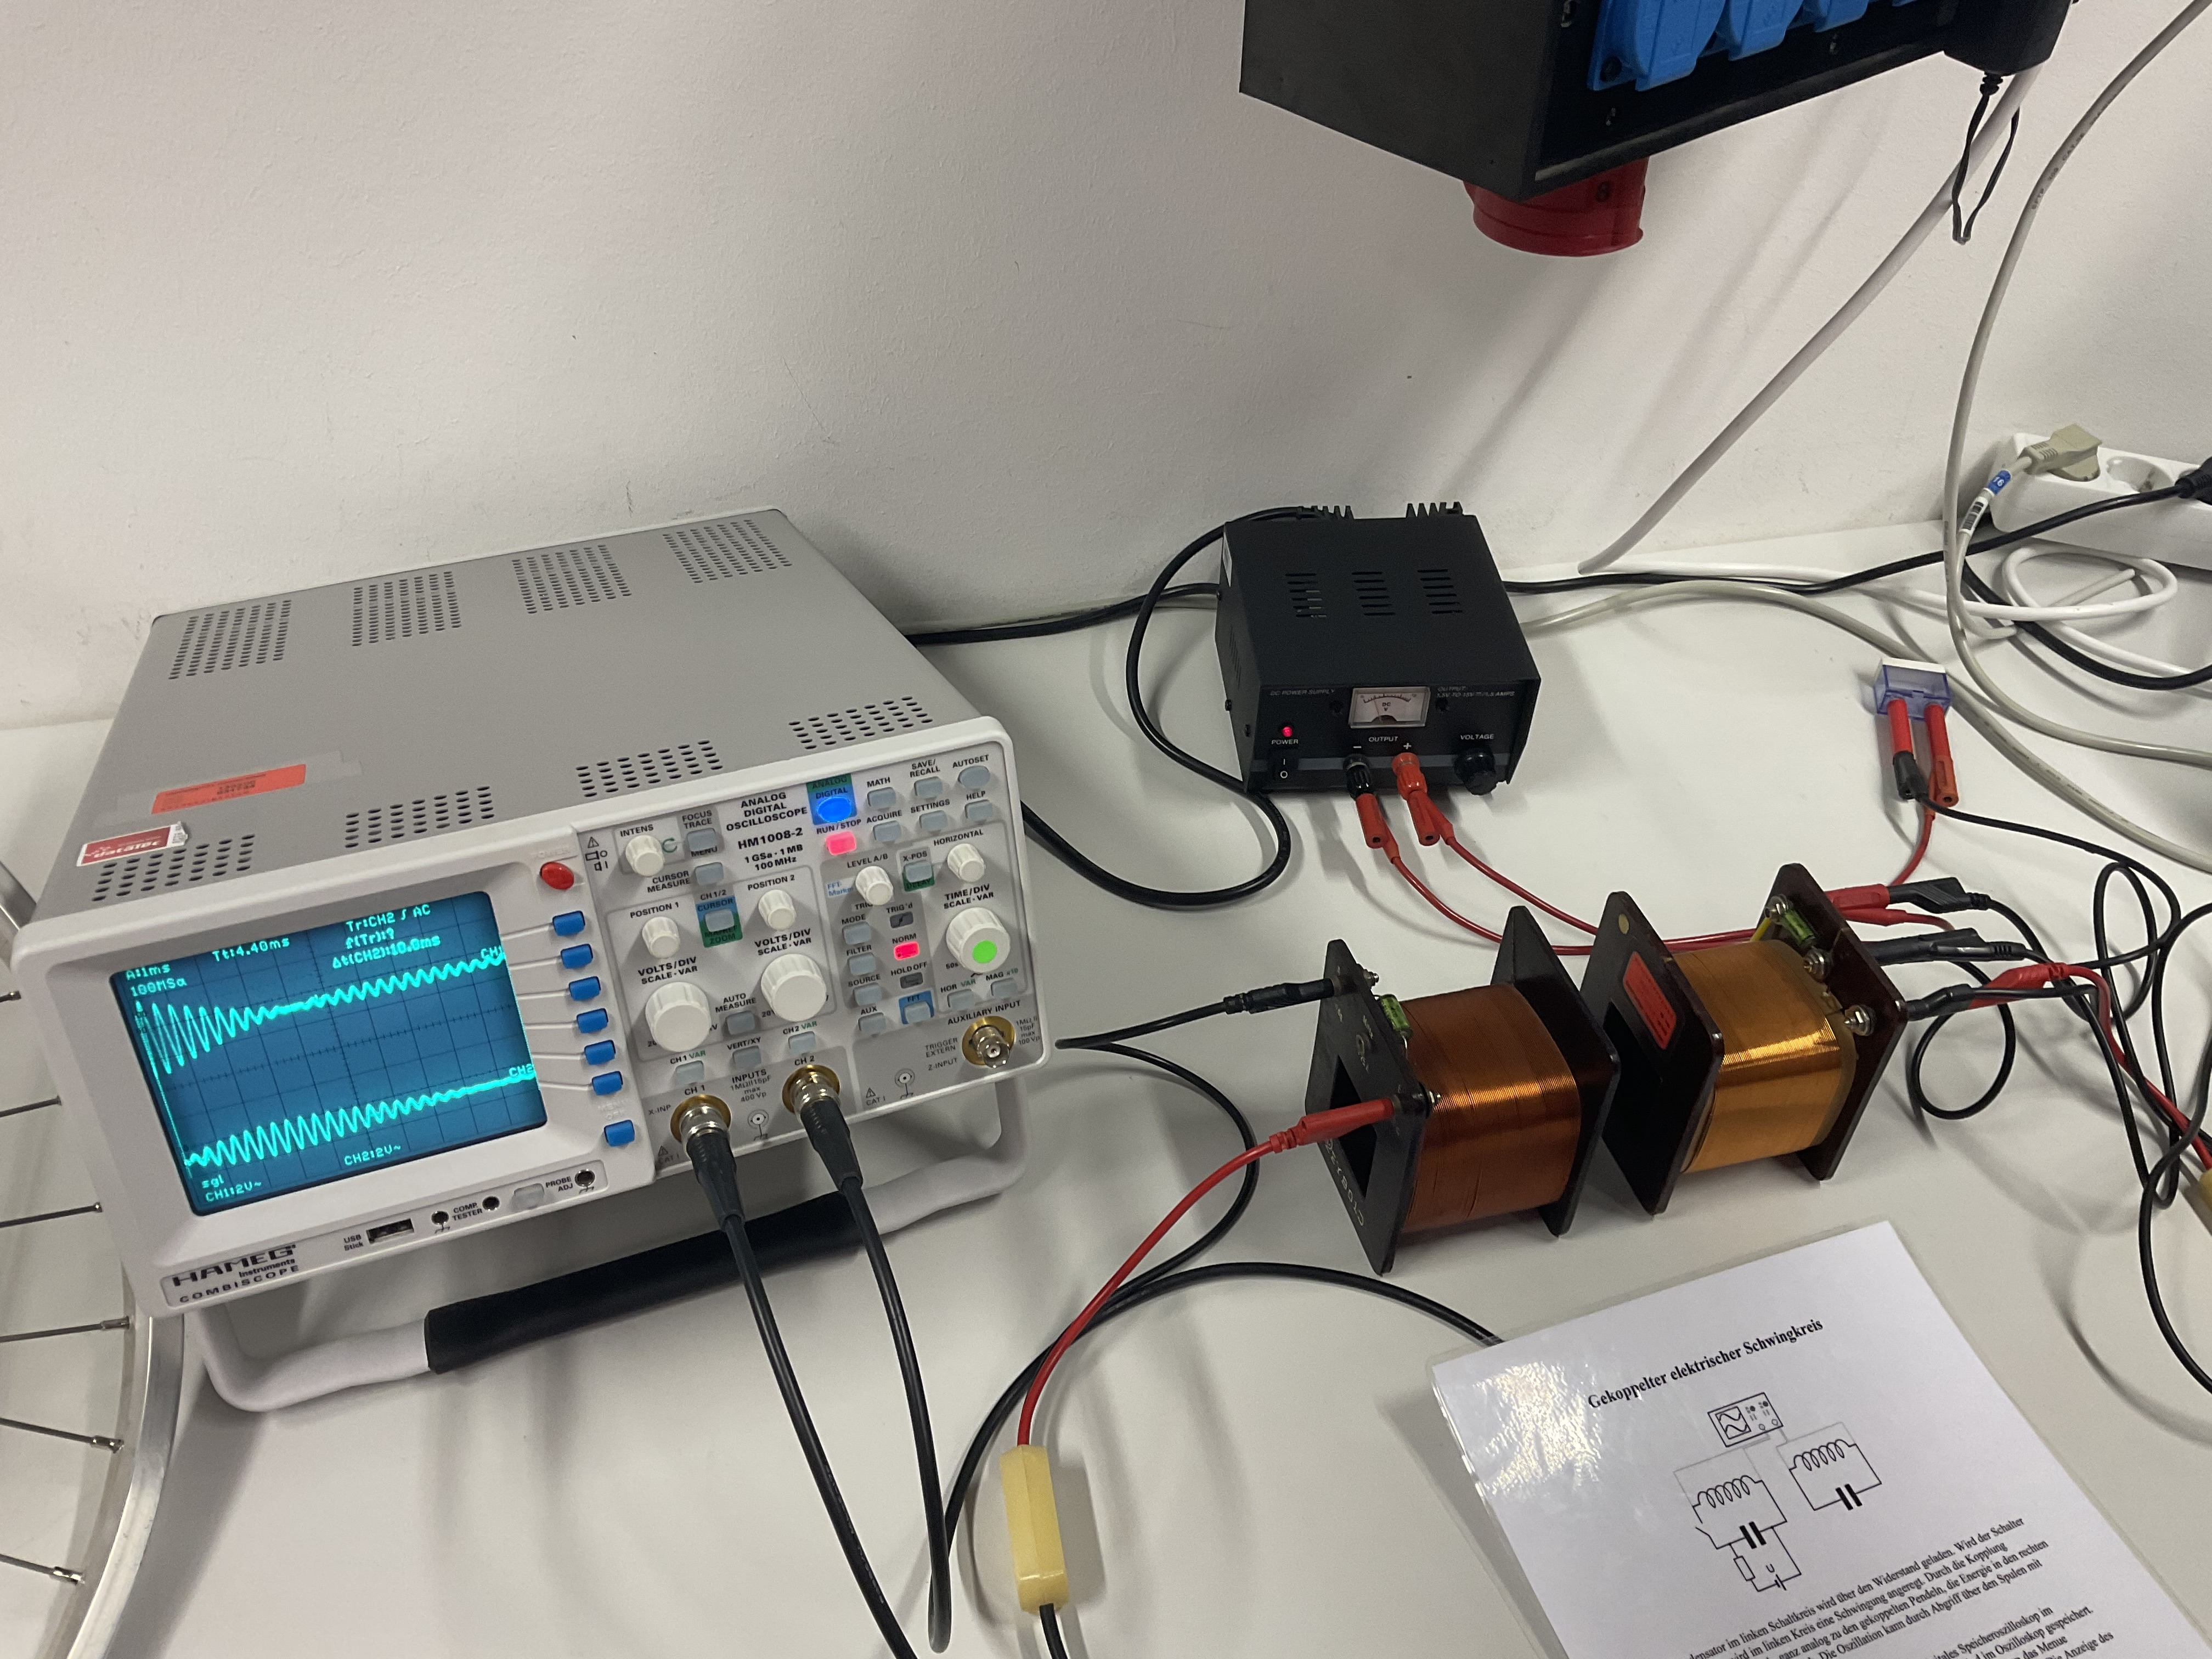
\includegraphics[width=0.48\textwidth]{graphics/IMG_0623.jpg}\label{fig:el_groß}}
  \hfill
  \caption{Konfigurationen des elektrischen Schwingkreises - verschiedene Abstände der Spulen}
  \label{fig:elSchw}
\end{figure}

\clearpage
\newpage
%-------------------------AUSWERTUNG-------------------------
\section{Auswertung}

In dieser Evaluation werden alle Fehler, sofern keine spezifische Angabe gemacht wird, mithilfe der Gauss'schen Fehlerfortpflanzung berechnet. Dies bedeutet, dass ein Wert $F$, der mit der Formel $f(a_1, ..., a_n)$ berechnet wird, den Fehler $\Delta F$ annimmt:

\begin{equation}
    \Delta F = \sqrt{\sum_n \left( \frac{\partial f}{\partial a_n} \cdot \Delta a_n \right)^2}.
\end{equation}

Des Weiteren erfolgen Signifikanztests von zwei Werten $a$ und $a'$ über die folgende Formel:

\begin{equation}
    \sigma = \frac{|a-a'|}{\sqrt{(\Delta a)^2 + (\Delta a')^2}}.
\end{equation}

Die Güte eines Fits wird mit der $\chi^2$-Summe bewertet:

\begin{equation}
    \chi^2 = \sum_i^N \left( \frac{\textit{Funktionswert}_i - \textit{Messwert}_i}{\textit{Fehler}_i} \right)^2
\end{equation}

Auch verwendet wird $\chi^2_{red} = \chi^2 / f$, wobei der Freiheitsgrad $f$ die Anzahl der Messwerte minus die Anzahl der Fitparameter ist. Der auf die Freiheitsgrade normierte Wert soll bei einem guten Fit ungefähr 1 sein.

\newpage

\subsection{Vergleich der reinen Frequenzen}

Zunächst betrachten wir die reinen Frequenzen, beginnend bei der Eigenschwingung der beiden Pendel ohne Kopplung. Der hier vom Gaußfit der Fouriertransformation berechnete Wert ist

\begin{equation}
    \omega_0 = (3,86 \pm 0,06) \frac{\text{rad}}{\text{s}},
\end{equation}

wobei der Fehler aus der Halbwertsbreite des Fits kommt. Analog lesen wir aus den Fits der symmetrischen und antisymmetrischen Schwingungen die Frequenzen für jede Kopplung aus. Dabei bezeichnet $\omega_1$ die symmetrischen und $\omega_2$ die antisymmetrischen Schwingungen. Da die symmetrische Schwingung unabhängig von der Kopplung ist, sollte sie für alle drei Kopplungsgrade die gleiche Frequenz wie das ungekoppelte Pendel mit $\omega_0$ aufweisen. Wir vergleichen also die Frequenzen $\omega_1$ mit $\omega_0$ über einen Signifikanztest und tragen alle berechneten Ergebnisse in Tabelle \ref{tab:reineFreq} ein.

\phantom{.}

\begin{table}[!h]
    \centering
    %\resizebox{\textwidth}{!}{
    \begin{tabular}{cccc}
        \hline
        \textbf{Kopplung} & $\bm{\omega_1}$ [rad/s]& $\bm{\omega_2}$ [rad/s]& $\bm{\sigma_{\omega_1, \omega_0}}$  \\ \hline
        schwach & $3,88 \pm 0,05$       & $3,98 \pm 0,06$ & $0,26$  \\
        mittel & $3,88 \pm 0,05$        & $4,17 \pm 0,06$ & $0,26$  \\
        stark & $3,88 \pm 0,05$         & $4,63 \pm 0,06$ & $0,26$  \\ \hline
    \end{tabular}%}
    \caption{Reine Frequenzen \& Vergleich von $\omega_0$ mit $\omega_1$}
    \label{tab:reineFreq}
\end{table}

\phantom{.}

Alle Signifikanztests weisen insignifikante Werte auf, somit stimmen die Frequenzen der ungekoppelten und der symmetrischen Schwingungen gut überein. Auch ist zu erkennen, dass die Frequenzen der asymmetrischen Schwingungen wie erwartet größer sind als die der symmetrischen Schwingungen und mit zunehmender Kopplungsstärke größer werden, was zu den theoretischen Erwartungen passt. Die Kopplung treibt wie erwartet die Schwingung an.

\newpage
\subsection{Vergleich der Schwebungsfrequenzen}

Wir beginnen, indem wir aus den durch die Gaußfits der Fouriertransformen bestimmten Frequenzen der Schwingungen die Werte von den Schwebungsschwingungen $\omega_I$ und $\omega_{II}$ bei jeder Kopplungsstärke bestimmen. Dazu ordenen wir erneut die Frequenz der symmetrischen Schwingung $\omega_1$ und die der antisymmetrischen $\omega_2$ zu und nutzen die gegeben Gleichungen für $\omega_I$ und $\omega_{II}$. Analog nutzen wir $\omega_1$ und $\omega_2$ der Fouriertransformierten der Schwebungsmessung. Der Fehler der Schwebungsfrequenzen ist gegeben als:  

\begin{equation}
    \Delta \omega_{I/II} = \frac{1}{2} \sqrt{(\Delta \omega_1)^2 + (\Delta \omega_2)^2}
\end{equation}

Die Ergebnisse sind in Tabelle \ref{tab:VGLfreq_AS_B} aufgetragen und über einen Signifikanztest werden die Werte aus den antisymmetrischen und symmetrischen Messungen mit denen der Schwebungsmessung verglichen. Der Index 'AS' bezeichnen die Werte der (anti-)symmetrischen Messungen und der Index 'B' die der Schwebungsmessung ('Beat').

\phantom{.}

\begin{table}[!h]
    \centering
    %\resizebox{\textwidth}{!}{
    \begin{tabular}{ccccc}
        \hline
        \textbf{Kopplung} & \textbf{Nr.} & $\bm{\omega_{AS}}$ [rad/s]& $\bm{\omega_B}$ [rad/s]& $\bm{\sigma}$  \\ \hline
        schwach & I & $3,93 \pm 0,04$       & $3,921 \pm 0,013$ & $0,15$  \\
        schwach & II & $0,05 \pm 0,04$  & $0,052 \pm 0,013$ & $0,024$  \\
        mittel & I & $4,02 \pm 0,04$        & $4,017 \pm 0,021$ & $0,14$  \\
        mittel & II & $0,15 \pm 0,04$     & $0,146 \pm 0,021$ & $0,023$  \\
        stark & I & $4,25 \pm 0,04$         & $4,248 \pm 0,022$ & $0,09$  \\
        stark & II & $0,38 \pm 0,04$        & $0,375 \pm 0,022$ & $10^{-14}$  \\ \hline
    \end{tabular}%}
    \caption{Vergleich berechneter Schwebungsfrequenzen - AS \& B}
    \label{tab:VGLfreq_AS_B}
\end{table}

\phantom{.}

Wie zu erkennen ist, sind alle Werte deutlich unterhalb der $1\sigma$-Grenze und passen somit gut zusammen. Zudem kann man erkennen, dass mit steigender Kopplungsstärke die Frequenzen ansteigen, was die Theorie bestätigt.

\phantom{.}

Wir wollen noch einen zweiten Vergleich machen, diesmal, indem wir manuell die Periodendauer der Schwebungswelle und den eingehüllten Wellen auslesen und somit die Frequenz berechnen:

\begin{equation}
    \omega = \frac{2 \pi}{T}, \ \ \ \ \ \Delta \omega = \frac{2 \pi}{T^2} \Delta T.
\end{equation}

Die Messungen der Periodendauern erfolgen über das Ablesen der Zeitpunkte zu Beginn $t_i$ und Ende $t_f$ einer Periode. Somit ergibt sich:

\begin{equation}
    T = t_f - t_i, \ \ \ \ \ \Delta T = \sqrt{(\Delta t_f)^2 + (\Delta t_i)^2}.
\end{equation}

Die Ergebnisse der Ausmessung sind in Tabelle \ref{tab:Perioden} verzeichnet. Es ist anzumerken, dass immer die Daten des ersten Pendels zur Ausmessung verwendet wurden.

\phantom{.}

\begin{table}[!h]
    \centering
    %\resizebox{\textwidth}{!}{
    \begin{tabular}{ccccc}
        \hline
        \textbf{Kopplung} & \textbf{Nr.} & $\bm{t_i}$ [s]& $\bm{t_f}$ [s] & $\bm{T}$ [s] \\ \hline
        schwach & I & $53,76 \pm 0,10$ & $55,37 \pm 0,10$ & $121,8 \pm 1,4$  \\
        schwach & II & $28,9 \pm 1,0$ & $150,7 \pm 1,0$ & $1,608 \pm 0,014$  \\
        mittel & I & $38,59 \pm 0,10$ & $40,16 \pm 0,10$ & $42,9 \pm 1,4$  \\
        mittel & II & $31,3 \pm 1,0$ & $74,2 \pm 1,0$ & $1,568 \pm 0,014$  \\
        stark & I & $21,79 \pm 0,10$ & $23,28 \pm 0,10$ & $17,0 \pm 1,4$  \\
        stark & II & $19,64 \pm 1,0$ & $36,6 \pm 1,0$ & $1,483 \pm 0,014$  \\ \hline
    \end{tabular}%}
    \caption{Ausmessung der Periodendauern}
    \label{tab:Perioden}
\end{table}

\phantom{.}

Aus den Periodendauern werden die Frequenzen berechnet (Index 'T') und diese mit den oben bestimmten Werten aus der Schwebung (Index 'B') verglichen.

\phantom{.}

\begin{table}[!h]
    \centering
    %\resizebox{\textwidth}{!}{
    \begin{tabular}{ccccc}
        \hline
        \textbf{Kopplung} & \textbf{Nr.} & $\bm{\omega_T}$ [rad/s]& $\bm{\omega_B}$ [rad/s]& $\bm{\sigma}$  \\ \hline
        schwach & I & $3,91 \pm 0,03$       & $3,921 \pm 0,013$ & $0,3$  \\
        schwach & II & $0,0516 \pm 0,0006$  & $0,052 \pm 0,013$ & $0,03$  \\
        mittel & I & $4,01 \pm 0,04$        & $4,017 \pm 0,021$ & $0,23$  \\
        mittel & II & $0,146 \pm 0,005$     & $0,146 \pm 0,021$ & $0,018$  \\
        stark & I & $4,24 \pm 0,04$         & $4,248 \pm 0,022$ & $0,26$  \\
        stark & II & $0,37 \pm 0,03$        & $0,0375 \pm 0,022$ & $0,12$  \\ \hline
    \end{tabular}%}
    \caption{Vergleich berechneter Schwebungsfrequenzen - T \& B}
    \label{tab:VGLfreq_T_B}
\end{table}

\phantom{.}

Auch hier liegen alle Abweichungen weit unterhalb der $1\sigma$-Grenze und sind somit wieder nicht signifikant.

\newpage
\subsection{Analyse der Kopplungsgrade}

Wir verwenden die bestimmten Frequenzen $\omega_1$ und $\omega_2$ der Schwebung sowie der symmetrischen und antisymmetrischen Schwingungen um die Kopplungsgrade der verschiedenen Federpositionen nach Formel \ref{eq:KopplGr_wT} zu berechnen. Für die schwache Kopplung ($D >> D'$) nähern wir diese Gleichung mit

\begin{equation}
    \kappa_{\sim} = \frac{D'}{D} = \frac{\omega^2_2 - \omega^2_1}{2\omega^2_1}.
\end{equation}

Damit bekommen wir für die genäherte und exakte Kopplung die Fehler:

\begin{equation}
    \begin{split}
        \Delta \kappa_{\sim} &= \kappa_{\sim} \sqrt{\left( \frac{\Delta \omega_2}{\omega_2} \right)^2 + \left( \frac{\Delta \omega_1}{\omega_1} \right)^2}, \\ \\
        \Delta \kappa &= \sqrt{\left( \frac{4 \omega^2_1 \omega_2}{(\omega^2_2 + \omega^2_1)^2} \Delta \omega_2 \right)^2 + \left( \frac{4 \omega^2_2 \omega_1}{(\omega^2_2 + \omega^2_1)^2} \Delta \omega_1 \right)^2}.
    \end{split}
\end{equation}

Wir bestimmen also die Kopplungsgrade einmal aus den Werten der Schwebung und einmal aus denen der symmetrischen und antisymmetrischen Schwingungen und bilden den Mittelwert aus beiden für unser Ergebnis.

\phantom{.}

\begin{table}[!h]
    \centering
    %\resizebox{\textwidth}{!}{
    \begin{tabular}{ccccc}
        \hline
        \textbf{Kopplung} & $\bm{\kappa_{AS}}$ & $\bm{\kappa_{B}}$ & $\bm{\kappa_{mean}}$  \\ \hline
        schwach & $0,026 \pm 0,020$       & $0,027 \pm 0,007$ & $0,026 \pm 0,010$  \\
        mittel & $0,072 \pm 0,019$        & $0,073 \pm 0,010$ & $0,072 \pm 0,011$  \\
        stark & $0,175 \pm 0,018$         & $0,175 \pm 0,010$ & $0,175 \pm 0,010$  \\ \hline
    \end{tabular}%}
    \caption{Kopplungsgrade aus gemessenen Frequenzen}
    \label{tab:kopplungsgrade_ws}
\end{table}

\phantom{.}

Wie zu erwarten nehmen die Kopplungsgrade für stärkere Kopplungen zu.

Wir betrachten nun das Verhältnis zweier Kopplungsgrade und erkennen, dass dieses aufgrund der Proportionalität von $D'$ zu $l^2$ gleich dem Verhältnis der Koppellängen ist:

\begin{equation}
    \frac{\kappa_1}{\kappa_2} = \frac{l^2_1}{l^2_2}
\end{equation}

Wir bestimmen also einmal das Verhältnis der eben berechneten Kopplungsgrade aus Tabelle \ref{tab:kopplungsgrade_ws} für die drei Möglichkeiten schwach/mittel, schwach/stark und mittel/stark sowie das Verhältnis der im Messprotokoll in Tabelle 1 aufgezeichneten Kopplungslängen und vergleichen diese mithilfe eines Signifikanztests. Die Fehler der Verhältnisse berechnen sich mit:

\begin{equation}
    \begin{split}
        \Delta \left( \frac{\kappa_1}{\kappa_2} \right) &= \frac{\kappa_1}{\kappa_2} \sqrt{\left( \frac{\Delta \kappa_1}{\kappa_1} \right)^2 + \left( \frac{\Delta \kappa_2}{\kappa_2} \right)^2} \\ \\
        \Delta \left( \frac{l^2_1}{l^2_2} \right) &= \frac{l^2_1}{l^2_2} \sqrt{\left( \frac{2 \cdot \Delta l_1}{l_1} \right)^2 + \left( \frac{2 \cdot \Delta l_2}{l_2} \right)^2}
    \end{split}
\end{equation}

\phantom{.}

\begin{table}[!h]
    \centering
    %\resizebox{\textwidth}{!}{
    \begin{tabular}{ccccc}
        \hline
        \textbf{Verhältnis} & $\bm{\frac{\kappa_1}{\kappa_2}}$ & $\bm{\frac{l^2_1}{l^2_2}}$ & $\bm{\sigma}$  \\ \hline
        schw/med    & $0,36 \pm 0,15$       & $0,3685 \pm 0,0028$ & $0,03$  \\
        schw/stark  & $0,15 \pm 0,06$       & $0,1455 \pm 0,0010$ & $0,07$  \\
        med/stark   & $0,41 \pm 0,07$       & $0,3949 \pm 0,0018$ & $0,28$  \\ \hline
    \end{tabular}%}
    \caption{Vergleich der Verhältnisse}
    \label{tab:vgl_verhältnisse}
\end{table}

\phantom{.}

Auch hier liegen alle Signifikanztests weit unterhalb der $1\sigma$-Grenze.

\subsection{Beobachtungen am Schwingungskreis}

In Abbildung \ref{fig:elSchw} sind die verschiedenen Konfigurationen des Schwingkreises und in den Bildern 1-3 des Messprotokolls die zugehörigen Aufnahmen der Schwingungen zu sehen. Man kann zunächst gut erkennen, dass bei einer stärkeren Kopplung, ergo dem Fall, wo die Spulen näher zusammen stehen, die Schwegungsfrequenz analog zum mechanischen Fall größer wird. Ebenso ist gut die Phasenverschiebung von $\frac{\pi}{2}$ zwischen den Schwebungen der einzelnen Schwingkreise zu erkennen. Wie zu erwarten sieht man also ein analoges Muster zum mechanischen Fall, was die Theorie bestätigt. 

\newpage
%---------------PRÄSENTATION DER ENDERGEBNISSE---------------
\section{Zusammenfassung der Endergebnisse}

In diesem Versuch wurden verschiedene Schwingarten eines gekoppelten Pendels untersucht, indem die Auslenkung in Abhängigkeit der Zeit von einer symmetrischen und antisymmetrischen Schwingung sowie einer Schwebung bei verschiedenen Kopplungseinstellungen aufgenommen wurde. Eine Fouriertransform der aufgezeichneten Signale mit Gaußfit ermöglichte eine Berechnung der Eigenfrequenzen der Schwingungen. 

Wir begannen, indem wir die reinen Schwingungsfrequenzen untersuchten. Hierbei wurde die bestimmte Frequenz der ungekoppelten Schwingung $\omega_0 = (3,86 \pm 0,06) \frac{\text{rad}}{\text{s}}$ als Referenz genutzt und mit den Frequenzen der symmetrischen Schwingung verglichen, die sich alle zu $\omega_1 = (3,88 \pm 0,05) \frac{\text{rad}}{\text{s}}$ ergaben. Der Vergleich über Signifikanztests ergab somit eine insignifikante Abweichung für alle Werte von 0,26. Zudem wurden die symmetrischen mit den antisymmetrischen Frequenzen verglichen und man konnte die erwartete Beobachtung machen, dass die asymmetrischen Sschwingungen höhere Frequenzen haben und diese mit stärkeren Kopplungen ansteigen, was auf die Abhängigkeit der asymmetrischen Schwingfrequenz vom Direktionsmoment der Kopplung zurückzuführen ist. 

Darauffolgend haben wir aus den aufgezeichneten Frequenzen die Schwebungsfrequenzen errechneten, einmal mit den Ergebnissen der symmetrischen und antisymmetrischen Schwingungen sowie mit den Ergebnissen der Schwebung. Beim Vergleich der jeweiligen Resultate lagen alle innerhalb insignifikanter Abweichungen voneinander und es konnte die Beobachtung gemacht werden, dass eine größere Kopplungsstärke eine höhere Frequenz ergibt. Auch konnte klar der Unterschied zwischen den Schwebungsfrequenzen $\omega_{II}$ und den Frequenzen der einzelnen Pendel $\omega_I$ aufgezeigt werden, indem zu erkennen ist, dass die einhüllenden Wellen mit einer kleineren Frequenz die eingehüllten, schnell oszillierenden Wellen umschließen.

Anschließend errechneten wir die Schwebungsfrequenzen aus manuell abgelesenen Periodendauern. Auch hier wies der Vergleich mit den vorher berechneten Werten nur insignifikante Abweichungen auf und es konnten die selben Beobachtungen wie zuvor gemacht werden.

Weiterhin berechneten wir dann noch die Kopplungsgrade aus den gemessenen Frequenzen und verglichen die Verhältnisse der Kopplungsgrade mit den Verhältnissen der Kopplungslängen. Erneut resultierten keine signifikanten Abweichungen und es konnte die theoretisch erwartete Beobachtung gemacht werden, dass eine stärkere Kopplung einen größeren Kopplungsgrad annimmt. Außerdem kann hier beobachtet werden, dass die Kopplung von schwach zu mittel und von mittel zu stark nicht linear zunimmt, was auch den Erwartungen entspricht, da das Direktionsmoment der Kopplung von den quadrierten Koppellängen abhängt und somit bei einer höheren Koppellänge quadratisch zunimmt. 

Abschließend werteten wir die Beobachtungen des elektrischen Schwingkreises aus und machten die erwarteten Beobachtungen. Analog zum mechanischen Fall wurden hier der Einfluss der Kopplungsstärke auf die Frequenz sowie die Phasenverschiebung in der Schwebung beobachtet.

\newpage
%---------------ZUSAMMENFASSUNG UND DISKUSSION---------------
\section{Diskussion}

Aufgrund der mehr als zufriedenstellenden Ergebnisse der Auswertung lässt sich schlussfolgern, dass alle Aspekte des Versuchs eindeutig und problemlos durchzuführen waren. Die Tatsache, dass der größte berechnete Sigma-Wert eines Signifikanztests bei 0,3 liegt und somit alle Werte deutlich innerhalb insignifikanter Abweichungen liegen ist eine eindeutige und aussagekräftige Bestätigung aller im Versuch untersuchten Theorien. Auch zeigt es, dass die Untersuchung eines gekoppelten Pendels mithilfe digitaler Software auf Basis des Hall-Effekts gut funktioniert und verlässliche Ergebnisse liefert. Überraschend waren vor allem die Ergebnisse der manuellen Ablesung der Periodendauern, hier hätten wir allein aufgrund des Fakts, dass man manuell etwas ablesen muss, durchaus größere Abweichungen erwartet, weshalb die guten Ergebnisse eine schöne Überraschung waren. Allgemein kann man sagen, dass die Verwendung digitaler Assistenz bei jedem Schritt von Durchführung bis Auswertung von großer Hilfe war. Eine Zurückerinnerung an das erste physikalische Anfängerpraktikum, wo ein Pendel manuell mit Stoppuhr und dem eigenhändigen Beobachten der Auslenkung analysiert wurde, zeigt wie sehr sich Messergebnisse verbessern, wenn zuverlässige digitale Geräte verwendet werden.

Allgemein lassen sich jedoch noch ein paar Anmerkungen zu theoretischen Fehlerquellen des Versuchs machen. Zunächst muss erwähnt werden, dass der Versuchsaufbau selbst die Pendel über die gemeinsame Aufhängung koppelt. Außerdem wird die Auslenkung per Hand im Allgemeinen wohl den größten Einfluss auf die Messwerte haben. Zum einen kann trotz bester Absicht nicht garantiert werden, dass bei den symmetrischen und antisymmetrischen Schwingungen die Pendel um den gleichen Winkel ausgelenkt werden. Dies ist auch bei uns daran zu sehen, dass bei den beiden aufgezeichneten Schwingungen leichte Schwebungen zu erkennen sind. Zudem kommt, dass die Pendel meist um einen recht großen Winkel ausgelenkt werden mussten, damit die Schwingungen über einen langer Zeitraum gemessen werden konnten, was die von uns gemachten Kleinwinkelnäherungen beim Aufstellen der Differentialgleichungen etwas ausreizt. Dennoch kann man trotz dieser Aspekten sagen, dass sie, obwohl sie wie die leichte Schwebung der symmetrischen und antisymmetrischen Schwingung teils sichtbar waren, bei uns nicht zu signifikanten Fehler geführt haben. 

Somit lässt sich abschließend sagen, dass der Versuch über die gesamte Bandbreite realistische und miteinander sehr gut verträgliche Ergebnisse geliefert hat und somit eine lehrreiche Einführung in die Grundlagen gekoppelter Schwingung darstellt.

\newpage
\includepdf[pages=-]{211-1.pdf}

\end{document}

